\subsubsection{Event Selection}

The jets in the analysis are reconstructed using the \antikt{} algorithm with a distance parameter $R=0.4$ and calibrated using the JES scheme (discussed in Section \ref{sec:Det:Jets}).
The analysis requires that a single jet trigger has passed.
Triggers are used if they are in the plateau region of the turn-on curve, corresponding to a greater than $99\%$ efficiency.
The trigger used for a given \ptave{} is shown in Table \ref{JetPerf:Triggers}.
A trigger with name jX requires an EF-level trigger jet with EM scale $\pt{}>$X GeV.
\begin{table}
%\footnotesize
\centering
\begin{tabular}{  c | c }
\hline
\hline
\ptave{} & Trigger\\
$[\rm GeV]$ & \\
\hline
$22-30$   & j10 \\
$30-40$   & j15 \\
$40-55$   & j20 \\
$55-75$   & j30 \\
$75-100$  & j40 \\
$100-130$ & j55 \\
$130-170$ & j75 \\
$170-220$ & j100 \\
$220-300$ & j135 \\
$300-400$ & j180 \\
\hline
\hline
\end{tabular}
\caption[Trigger strategy for dijet \pt{} balance in 2011]{
Trigger strategy for the different dijet \ptave{}. 
\label{JetPerf:Triggers}}
\end{table}
The data are required to be in luminosity blocks when all ATLAS sub-detectors are fully functioning. 

To ensure the $2\rightarrow2$ scattering topology the \dphi{} between the two jets is required to be greater than $2.5$ rad and events containing a third jet with $\pt{} >0.25~ \ptave{}$ are removed.
The reference region that is used to do the final rescaling of the responses in the matrix method is \etarange{-0.8}{0.8}.

\subsubsection{Basic Asymmetry and Response Distributions}

Figures \ref{JetPerf:Asym_j15} and \ref{JetPerf:Asym_j30} each show two asymmetry distributions for jets falling in (a) two central regions, $-0.8<\eta_{left}<-0.1$ and $0.1<\eta_{right}<0.8$, and (b) one central region and one more forward region, $0.1<\eta_{left}<0.8$ and $2.1<\eta_{right}<2.8$. 
Each asymmetry distributions have been fitted with a Gaussian function from $-0.7<\mathcal{A}<0.7$.

Figure \ref{JetPerf:Asym_j15} shows asymmetry distributions for $30<\ptave{}<40$ GeV jets.
The peak of the fitted asymmetry for both jets falling in the central region is $0.006$, which corresponds to a very small \pt{} imbalance of $\mean{\pt{}^{right}}= 0.994 \mean{\pt{}^{left}}$.
The peak of the fitted asymmetry for one jet falling in the central region and the other in a forward region is $0.023$, which corresponds to a \pt{} imbalance of $\mean{\pt{}^{right}}= 0.98 \mean{\pt{}^{left}}$.

Figure \ref{JetPerf:Asym_j30} shows asymmetry distributions for $55<\ptave{}<75$ GeV jets.
The peak of the fitted asymmetry for both jets falling in the central region is $0.003$, which corresponds to very small \pt{} imbalance of $\mean{\pt{}^{right}}= 0.997 \mean{\pt{}^{left}}$. 
The peak of the fitted asymmetry for one jet falling in the central region and the other in a forward region is $0.007$, which corresponds to a \pt{} imbalance of $\mean{\pt{}^{right}}= 0.993 \mean{\pt{}^{left}}$.

The width in the asymmetry distributions arises due to the jet energy resolution of the two jets and the peak value of the fitted asymmetry relates to the relative responses of the two regions.
In the distributions for both the low and high \ptave{} jets, the case where both jets fall into central regions has a lower \pt{} imbalance than the case where one jet falls into a forward region.  
When both jets fall into the barrel region they are better calibrated, as the barrel region is well understood (through test beam information and single hadron response) and has little dead material.
However, when one jet is further forward, is falls into the end-cap region of the calorimeter and the difference observed could be due to the differing abilities to calibrate the different parts of the detector. 
The spread of asymmetry is smaller for higher \ptave{} jets, which is due to the improved resolution for higher \pt{} jets.


Figures \ref{JetPerf:ResponseMatrix_30_40_j15} and \ref{JetPerf:ResponseMatrix_55_75_j30} show the the response matrices, which are used by the minimisation, for jets in the range $30<\ptave{}<40$~GeV and $55<\ptave{}<75$ GeV, respectively.
The low \ptave{} jets have a larger range of relative responses than the high \ptave{} jets, with some bins deviating from unity by up to $6\%$.
In both response matrices the higher $\eta$ bins have a larger spread of responses than the more central bins.


Figure \ref{JetPerf:PtComp} shows the relative response as a function of detector $\eta$ for $22<\ptave{}<30$ GeV jets, $30<\ptave{}<40$ GeV jets, and $55<\ptave{}<75$ GeV jets. 
The largest relative response occurs for low \ptave{}.
There is a relative response of about $1.02$ at $|\eta|=1$ which corresponds to the crack region between the tile barrel and tile extended barrel. 
This crack can be seen in the jet energy EM-scale response in Figure \ref{Det:MCResp}.
For low \pt{} jets, the calibration has over-calibrated the jets in this crack region. 
For the medium and high jet \pt{} ranges shown, the relative response for $|\eta|<1$ is very close to unity.
The response at higher $\eta{}$ deviates away from unity, and as the jet \pt{} increases this deviation reduces. 

\begin{figure}
\centering
        \begin{subfigure}[b]{0.8\textwidth}
                \centering
                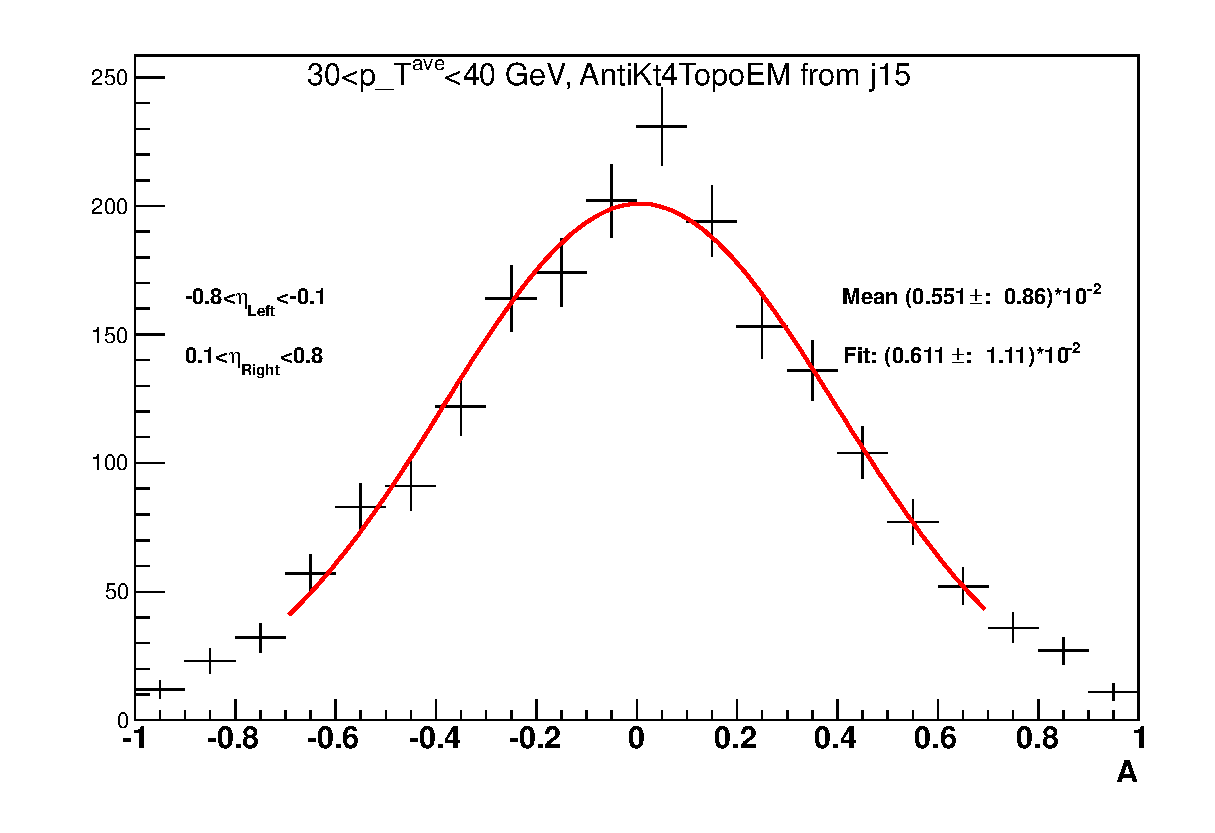
\includegraphics[width=\textwidth]{figures/JetPerformance/2011/j15zvar4_6.eps}
        \end{subfigure}%

        \begin{subfigure}[b]{0.8\textwidth}
                \centering
                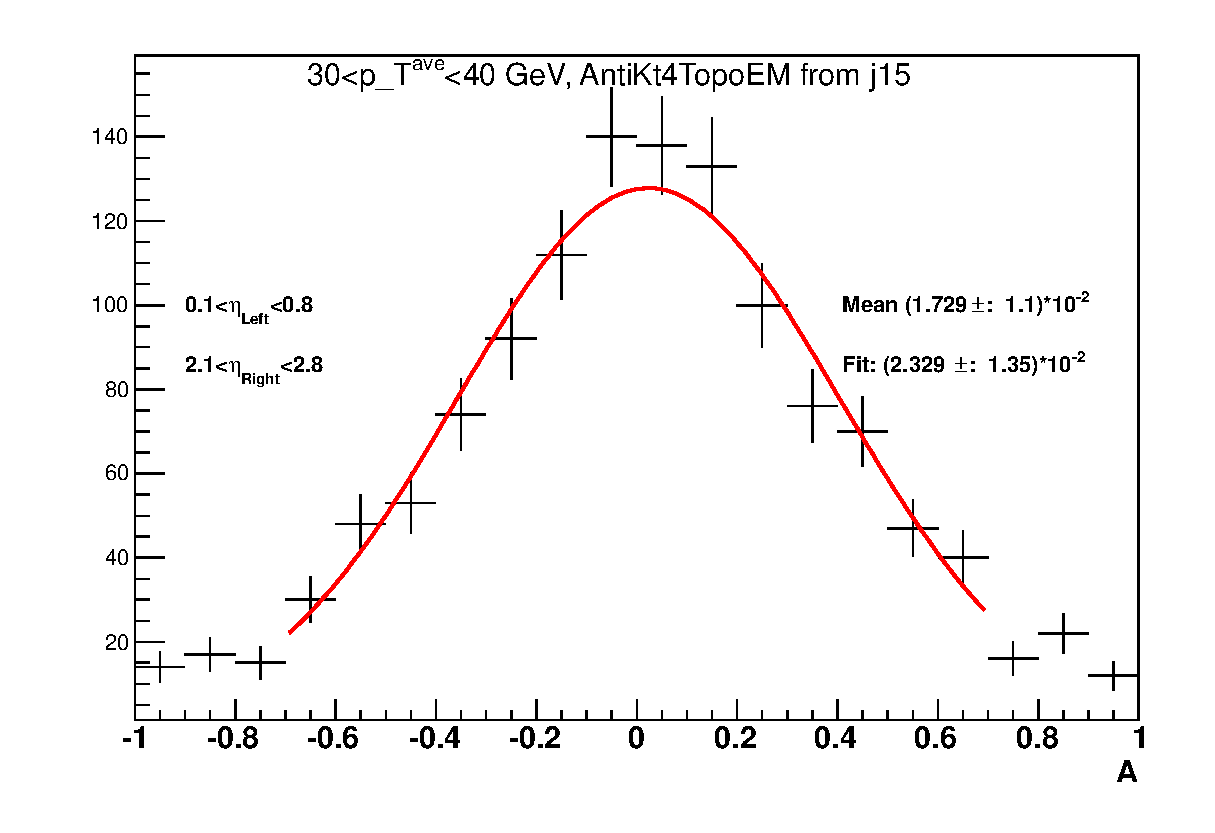
\includegraphics[width=\textwidth]{figures/JetPerformance/2011/j15zvar6_9.eps}
        \end{subfigure}%
\caption[Example asymmetry distribution for jets with $30<\ptave{}<40$ GeV]{
Asymmetry distribution for jets with $30<\ptave{}<40$ GeV with (a) $-0.8<\eta_{left}<-0.1$ and $0.1<\eta_{right}<0.8$ and (b)  $0.1<\eta_{left}<0.8$ and $2.1<\eta_{right}<2.8$.
The distribution is fitted using a Gaussian function between $\rm{-0.7<A<0.7}$ and the fit result and error is shown as is the mean and error on the mean. 
\label{JetPerf:Asym_j15}}
\end{figure}

\begin{figure}
\centering
        \begin{subfigure}[b]{0.8\textwidth}
                \centering
                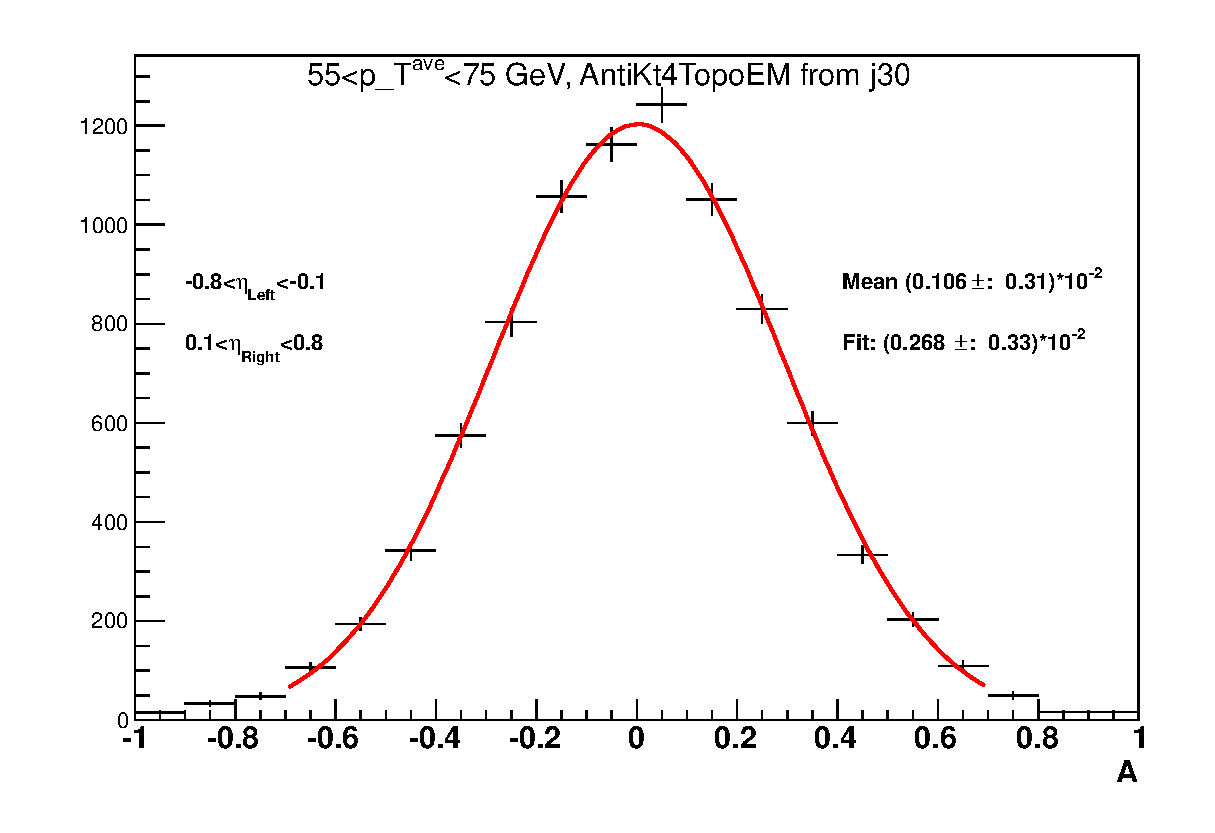
\includegraphics[width=\textwidth]{figures/JetPerformance/2011/j30zvar4_6.eps}
        \end{subfigure}%

        \begin{subfigure}[b]{0.8\textwidth}
                \centering
                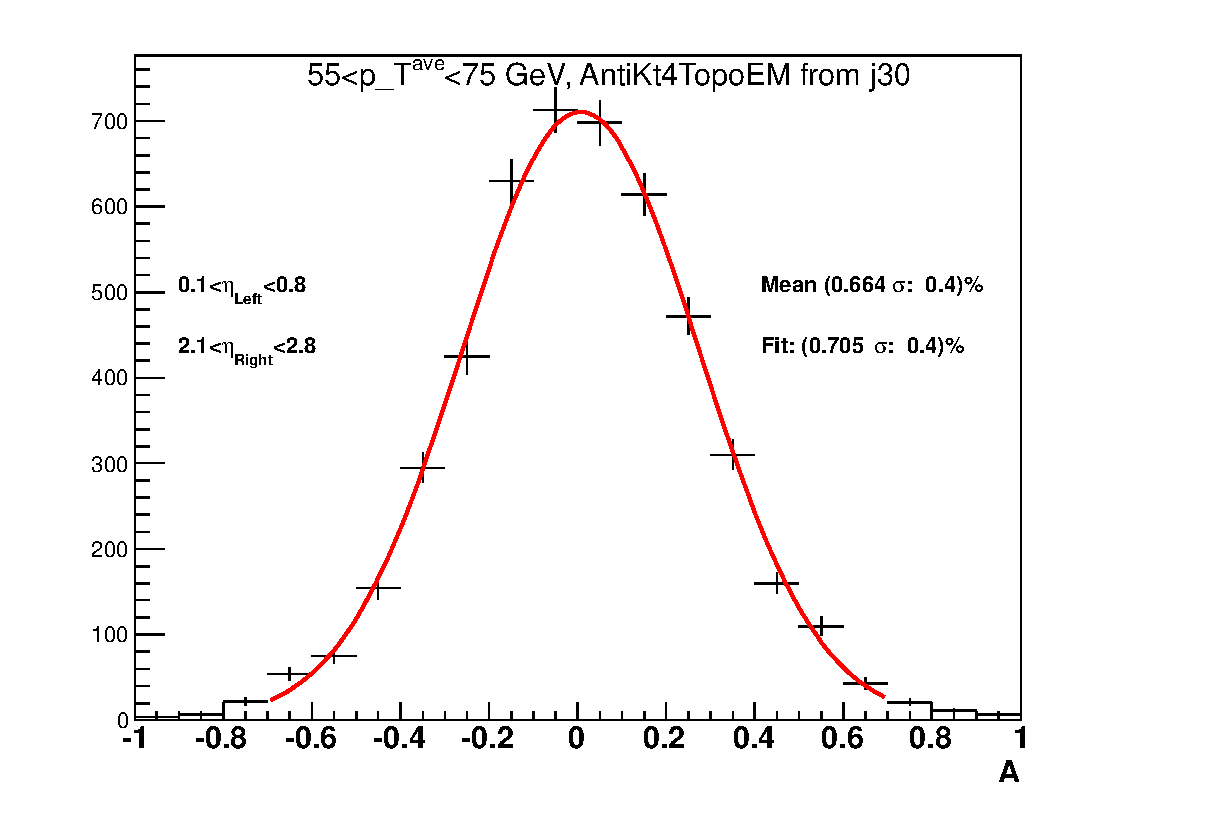
\includegraphics[width=\textwidth]{figures/JetPerformance/2011/j30zvar6_9.eps}
        \end{subfigure}%

\caption[Example asymmetry distribution for jets with $55<\ptave{}<75$ GeV]{
Asymmetry distribution for jets with $55<\ptave{}<75$ GeV with (a) $-0.8<\eta_{left}<-0.1$ and $0.1<\eta_{right}<0.8$ and (b)  $0.1<\eta_{left}<0.8$ and $2.1<\eta_{right}<2.8$.
The distribution is fitted using a Gaussian function between $\rm{-0.7<A<0.7}$ and the fit result and error is shown as is the mean and error on the mean. 
\label{JetPerf:Asym_j30}}
\end{figure}

\begin{figure}
\centering
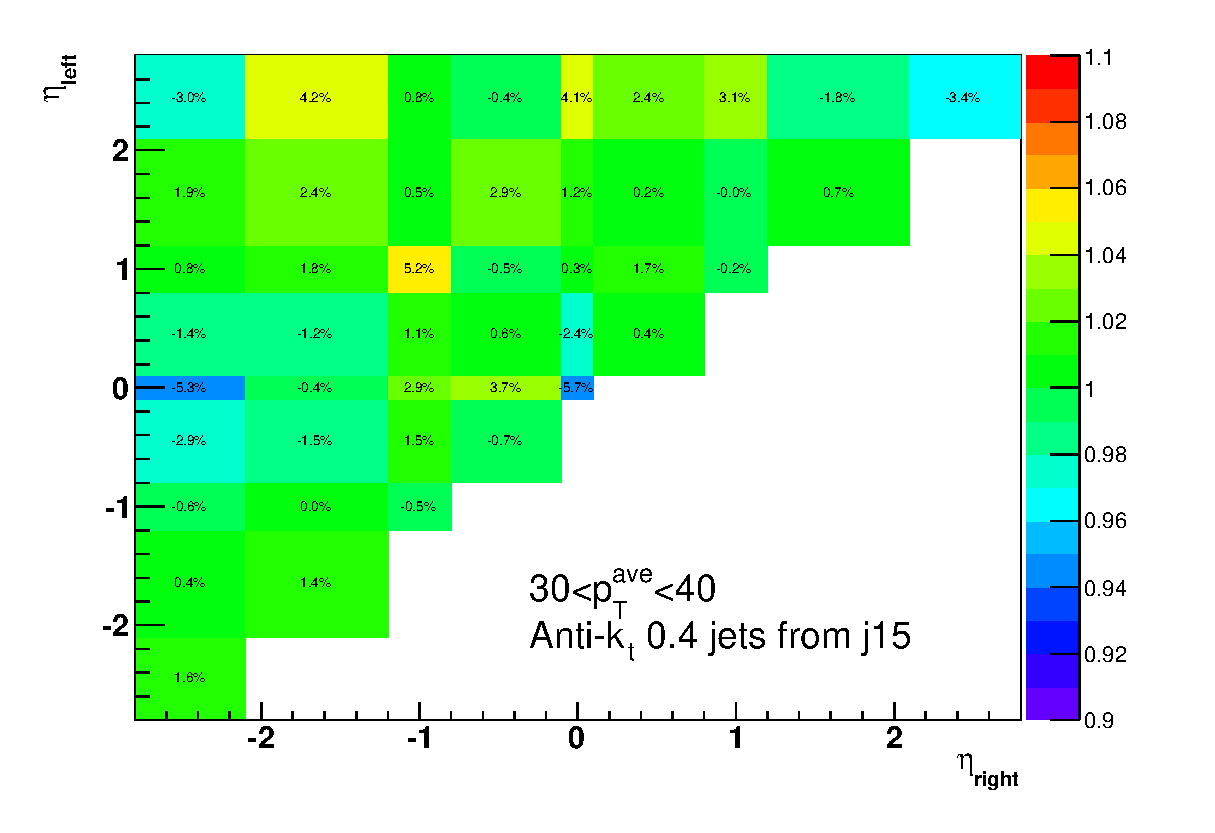
\includegraphics[width=0.9\textwidth]{figures/JetPerformance/2011/j15TwoDPlotBoth.eps}
\caption[The response matrix for jets with $30<\ptave{}<40$ GeV]{
Response matrix for $30<\ptave{}<40$ GeV for jets which passed the j15 trigger. 
The text in the bins corresponds to the percentage difference between the response and unity.
\label{JetPerf:ResponseMatrix_30_40_j15}}
\end{figure}

\begin{figure}
\centering
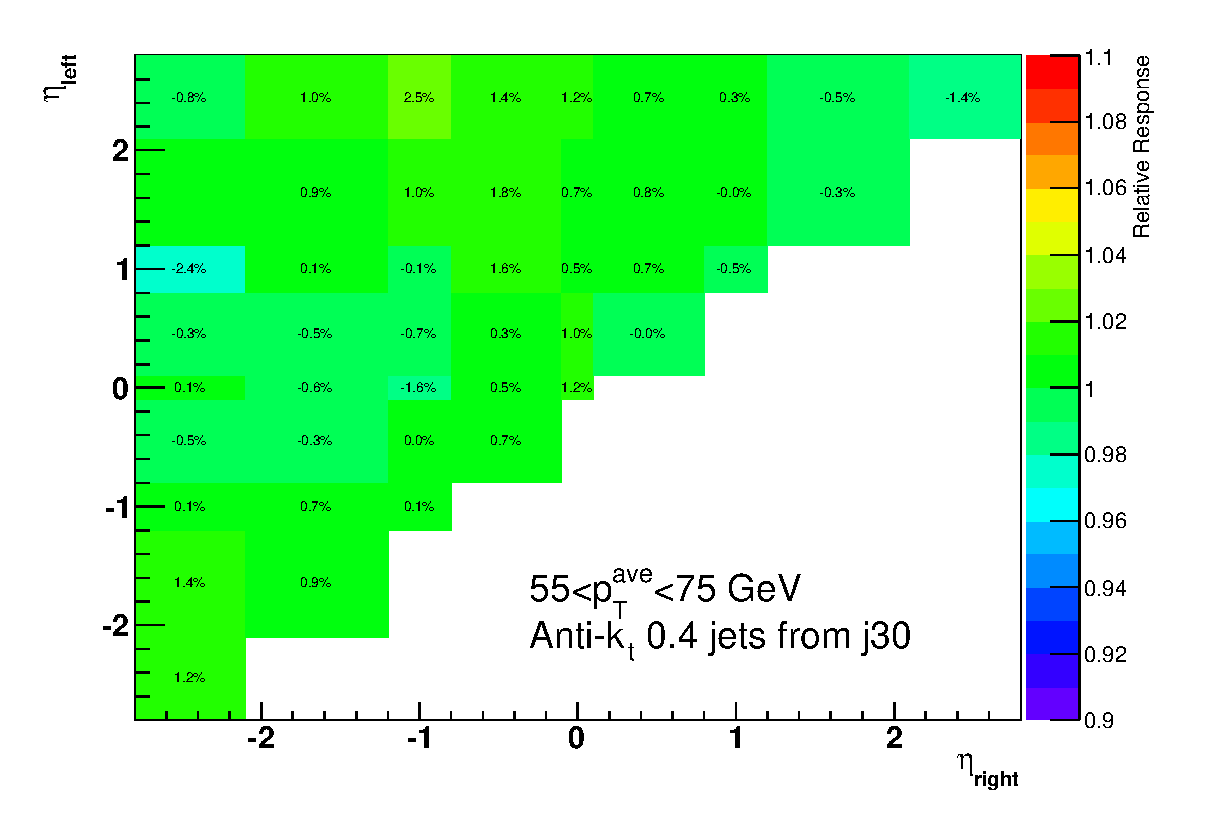
\includegraphics[width=0.9\textwidth]{figures/JetPerformance/2011/j30TwoDPlotBoth.eps}
\caption[The response matrix for jets with $55<\ptave{}<75$ GeV]{
Response matrix for $55<\ptave{}<75$ GeV for jets which passed the j30 trigger. 
The text in the bins corresponds to the percentage difference between the response and unity.
\label{JetPerf:ResponseMatrix_55_75_j30}}
\end{figure}


\begin{figure}
\centering
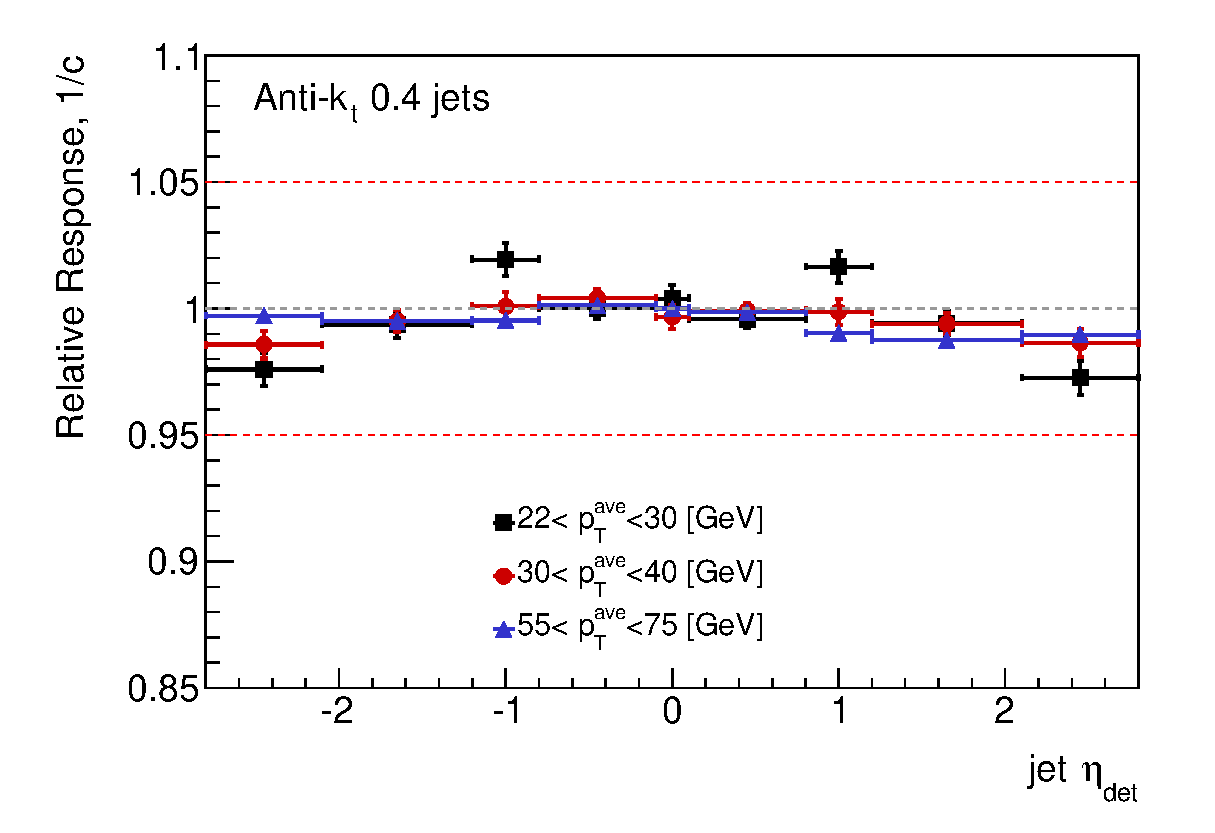
\includegraphics[width=0.9\textwidth]{figures/JetPerformance/2011/ResponseAvePtComp.eps}
\caption[Relative response as a function of $\eta$]{
Relative response as a function of detector $\eta$ for jets with $22<\ptave{}<30$ GeV, $30<\ptave{}<40$ GeV and $55<\ptave{}<75$ GeV.
\label{JetPerf:PtComp}}
\end{figure}


